% \chapter{Trigonometry}
% Trigonometry relates angles and lengths of triangles. Figure \ref{fig:triangle} shows a right-angled triangle and conventions to label its corners, sides, and angles. In the following, we assume all triangles to have at least one right angle (90 degrees or $\frac{\pi}{2})$ as all planar triangles can be dissected into two right-angled triangles. 

\chapter{三角学}
三角法涉及三角形的角度和长度。图\ref{fig:triangle}显示了一个直角三角形和约定来标记其角,边和角度。在下文中,我们假设所有三角形都具有至少一个直角(90度或$\frac{\pi}{2})$,因为所有平面三角形都可以解剖成两个直角三角形。

\begin{figure}[!htb]
\centering
\includegraphics[width=0.8\textwidth]{figs/triangle}
% \caption{Left: A right-angled triangle with common notation. Right: Trigonometric relationships on the unit circle and angles corresponding to the four quadrants. \label{fig:triangle}}
\caption{左:具有常用符号的直角三角形。 右:单位圆上的三角关系和对应于四个象限的角度。}
\label{fig:triangle}
\end{figure}

% The sum of all angles in any triangle is 180 degrees or $2\pi$, or 

任何三角形中所有角度的总和为180度或$2\pi$,或

\begin{equation}
\alpha + \beta + \gamma = 180^o
\end{equation}

% If the triangle is right-angled, the relationship between edges $a$, $b$, and $c$, where $c$ is the edge opposite of the right angle is

如果三角形是直角的,则边缘之间的关系$a$,$b$和$c$,其中$c$是与直角相反的边缘

\begin{equation}
a^2+b^2=c^2
\end{equation}

% The relationship between angles and edge lengths are captured by the trigonometric functions:

角度和边缘长度之间的关系由三角函数捕获:

\begin{eqnarray}
\sin{\alpha}&=\frac{opposite}{hypothenuse}=\frac{a}{c}\\
\cos{\alpha}&=\frac{adjacent}{hypothenuse}=\frac{b}{c}\\
\tan{\alpha}&=\frac{opposite}{adjacent}=\frac{\sin{\alpha}}{\cos{\alpha}}=\frac{a}{b}
\end{eqnarray} 

% Here, the \emph{hypothenuse}\index{Hypothenuse} is the side of the triangle that is opposite to the right angle. The \emph{adjacent} and \emph{opposite} are relative to a specific angle. For example, in Figure \ref{fig:triangle}, the adjacent of angle $\alpha$ is side $b$ and the opposite of $\alpha$ is edge $a$. 

% Relations between a single angle and the edge lengths are captured by the \emph{law of cosines}\index{Law of Cosines}:

这里,\emph{hypothenuse}\index{Hypothenuse}是三角形与正确角度相反的一面。\emph{adjacent}和\emph{opposite}相对于特定角度。例如,在图\ref{fig:triangle}中,角度$\alpha$的相邻边是$b$,而$\alpha$的相反是边缘$a$。

单个角度和边缘长度之间的关系由\emph(余弦定律)\index{余弦定律}捕获:

\begin{equation}
a^2=b^2+c^2-2bc\cos{\alpha}
\end{equation}

% \section{Inverse trigonometry}
% In order to calculate an angle given two edges, one uses inverse functions $\sin^{-1}$, $\cos^{-1}$, and $\tan^{-1}$. (Not to be confused with $\frac{1}{\sin}$ etc.) As functions can, by definition, only map one value to exactly one other value, $\sin^{-1}$ and $\tan^{-1}$ are only defined in the interval $[-90^o;+90^o]$ and $\cos^{-1}$ is defined in the interval $[0^o;180^o]$. This makes it impossible to calculate angles in the 2nd and 3rd, or the 3rd and 4th quadrant, respectively (Figure \ref{fig:triangle}). 
% In order to overcome this problem, most programming languages implement a function \texttt{atan2(opposite,adjacent)}, which evaluates the sign of the numerator and denumerator, provided as two separate parameters. 

\section{逆三角}
为了计算给定两个边的角度,一个使用逆函数$\sin^{-1}$,$\cos^{-1}$和$\tan^{-1}$。(不要与$\frac{1}{\sin}$等混淆)因为根据定义,函数只能将一个值映射到一个其他值,$\sin^{-1}$和$\tan^{-1}$仅在间隔$[-90^o;+90^o]$和$\cos^{-1}$中定义在间隔$[0^o;180^o]$。这使得不可能分别计算第2和第3或第3和第4象限的角度(图\ref{fig:triangle})。
为了克服这个问题,大多数编程语言都实现了一个函数\texttt{atan2(相对的,相邻的)},它计算了分子和数组的符号,它们被提供为两个单独的参数。

% \section{Trigonometric identities}
% Sine and cosine are periodic, leading to the following identities:

\section{Trigonometric identity}
正弦和余弦是周期性的,导致以下身份:

\begin{eqnarray}
\sin\theta=-\sin(-\theta)=-\cos(\theta+\frac{\pi}{2})=\cos(\theta-\frac{\pi}{2})\\
\cos\theta=\cos(-\theta)=\sin(\theta+\frac{\pi}{2})=-\sin(\theta-\frac{\pi}{2})
\end{eqnarray}

% The sine or cosine for sums or differences between angles can be calculated using the following identities:

可以使用以下身份计算角度之和或正差或正弦:

\begin{eqnarray}
\cos(\theta_1+\theta_2)=\cos(\theta_1)\cos(\theta_2)-\sin(\theta_1)\sin(\theta_2)\\
\sin(\theta_1+\theta_2)=\sin(\theta_1)\cos(\theta_2)+\cos(\theta_1)\sin(\theta_2)\\
\cos(\theta_1-\theta_2)=\cos(\theta_1)\cos(\theta_2)+\sin(\theta_1)\sin(\theta_2)\\
\sin(\theta_1-\theta_2)=\sin(\theta_1)\cos(\theta_2)-\cos(\theta_1)\sin(\theta_2)
\end{eqnarray}

% The sum of the squares of sine and cosine for the same angle is one:

相同角度的正弦和余弦的平方和之和为1:

\begin{equation}
\cos(\theta)\cos(\theta)+\sin(\theta)\sin(\theta)=1
\end{equation}